% Activate the following line by filling in the right side. If for example the name of the root file is Main.tex, write
% "...root = Main.tex" if the chapter file is in the same directory, and "...root = ../Main.tex" if the chapter is in a subdirectory.
 
%!TEX root =  mainMastersProject.tex

\chapter[Simple Non-Spatial Simulations]{A Simple Stabbing - Non-Spatial Simulations and their Bayesian Networks}

\section{Introduction}
Here I talk about the credibility game and Charlotte Vlek's Stabbing Bayesian Network example.

In these non-spatial simulations, there are agents, and they interact with each other, but there is no environment for them to interact in. So the simulation is a pure combination of the probabilities assigned to each state transition (or something along those lines). In a sense, the probability for an agent to `stab with knife' purely depends on the probability of `motive' and `opportunity'. Compared to a spatial simulation, where `opportunity' is more complex, as it involves proximity to victim which arises from the simulation and not from some random number generator.

These non-spatial simulations are boring, but they are necessary first steps: after all, if we cannot make BNs out of these predetermined (the probabilities in each run are not predetermined, but the distributions that they are drawn from, and their thresholds, are), then the rest of our endeavours will be fruitless. On the other hand, if the process for creating and evaluating these simple simulations work well, then we can proceed to modelling more complex, spatial simulations.

In this part, I have two experiments. One simple experiment meant to be a replication of Charlotte Vlek's Bayesian Network in xxx \footnote{rephrase}, and another simple experiment mainly meant to test the evaluation criteria for the Bayesian Networks, as outlined in the previous chapter.

\section{Method}
%There are two methods outlined here, one for each initial experiment.

\subsection{Vlek Networks}
Take the Vlek networks from Vlek Jurix 2015.

The general story is: Jane and Mark had a fight, but Jane had a knife. Mark died. 

Then, there are two specific scenarios that can explain why Mark died. In scenario one, Jane stabbed Mark, and then he died. In scenario 2, Jane threatened Mark with the knife, Mark hit Jane, Jane dropped the knife, Mark fell on the knife, and Mark died by accident. There are two separate networks for these scenarios.

I'm going to create two separate networks, and then also see if I can merge them, by creating a Jane-and-Mark-knife simulation, assigning some random probabilities that correspond to the story, and see what the K2 algorithm makes of it. Then I will also merge the two networks to see if the K2 can deal with mutually exclusive nodes (eg: `Mark died by accident' should rule out `Mark died by stabbing').

So, I created some logical rules, either atoms or rules, and we can process in the simulation these using standard forward chaining inference. Every atom has a prior probability, and every conclusion of a rule has a probability given the F/T state of the premises. At every step, the simulation checks which new sentences are true, applies a rule with a given probability, and counts the outcome.

This does mean that rules at the end are not triggered as often as rules in the beginning, even if they have the same trigger probability (they are on other sides of the chain, more needs to be have happened to conclude that Mark died).

\subsection{Behavioural rules for the simulation}

Global

\textbf{Jane and Mark had a fight} (80, 20)

\textbf{Jane had a knife} (30, 70)


Scenario 1


\textbf{Jane had a knife} and \textbf{Jane and Mark had a fight} $\rightarrow$ \textbf{Jane stabbed Mark with a knife} (99, 1) (1, 0)

\textbf{Jane stabbed Mark with a knife} $\rightarrow$ \textbf{Mark died} (20, 80)

Scenario 2

\textbf{Jane had a knife} and \textbf{Jane and Mark had a fight} $\rightarrow$ \textbf{Jane threatened Mark with a knife} (97, 3) (1, 0)

\textbf{Jane threatened Mark with a knife} $\rightarrow$  \textbf{Mark hit Jane} (5, 95)

\textbf{Jane dropped the knife} $\rightarrow$ \textbf{Mark fell on the knife} (99, 1)

\textbf{Mark fell on the knife} $\rightarrow$ \textbf{Mark died by accident} (40, 60)

 \textbf{Mark died by accident} $\rightarrow$  \textbf{Mark died}  (0, 100)

This was done using forward chaining, with a time index, which means that a rule could only be triggered at one time (otherwise the probabilities get messed up). So we have a forward chaining rule, which means that if the premises of some rule are true, there are no excluding facts true, the timestep is correct, and the random number generator generated a number that is lower than the probability threshold, we find that the conclusion is true, and add it to our found facts. We keep doing this.


Since Vlek does not give probabilities in her paper, I'm just making some up. The logical sentences are reporters in the simulation, and then I let the simulation run for many times (10,000 times). Then there came out three different Bayesian Networks, one for scenario 1, one for scenario 2, and one for the combined network (Figure~\ref{kb1}, Figure~\ref{kb2}, Figure~\ref{full}).

\begin{figure}[htbp]
\begin{center}
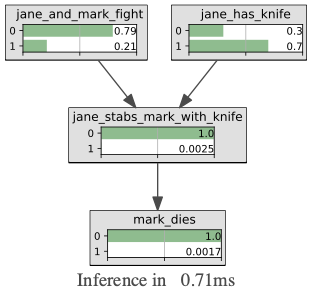
\includegraphics[scale = 0.5]{images/Kb1.png}
\caption{Automatically generated BN with K2 and the above forward chaining rules, scenario 1.}
\label{kb1}
\end{center}
\end{figure}

\begin{figure}[htbp]
\begin{center}
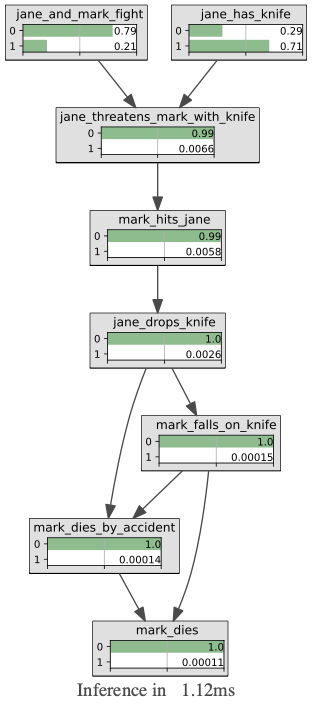
\includegraphics[scale = 0.5]{images/Kb2.png}
\caption{Automatic generated BN with K2 and above forward chaining rules, scenario 2}
\label{kb2}
\end{center}
\end{figure}

\begin{figure}[htbp]
\begin{center}
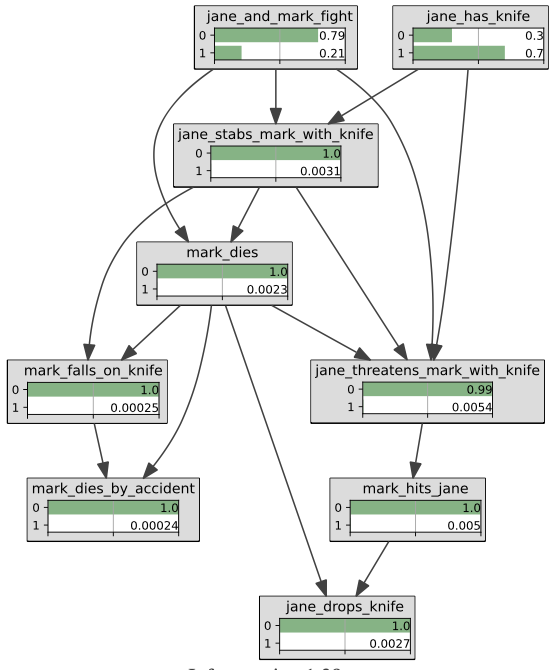
\includegraphics[width=\linewidth]{images/Kb.png}
\caption{Automatically generated BN with rules from both scenarios included.}
\label{full}
\end{center}
\end{figure}

\section{Results - Figure comparison to Vlek 2015}
If we only look at the ordering of the Bayesian Network, we can see that for Figure~\ref{kb1}, the sub-scenario structure is the same as in Vlek 2015 Figure~3. There's no scenario node constraining the network, all the information is contained in the network, no scenario node needed (todo: make the nodes the exact same names).

However, there are differences between Vlek 2015 Figure~4, and the automatically generated BN here. Figure~4 in Vlek 2015 is replicated below in Figure~\ref{vlek} (todo: ask permission?? or just remove). The automatically generated BN is very linear and can be interpreted in a purely temporal way: mark hits jane, jane drops the knife, and due to jane dropping the knife, and mark falling on it, mark dies by accident - and if mark dies by accident, mark dies. The probabilities for all these events (from jane dropping the knife on), are ridiculously low, and don't really make sense (should interpret the small probabilities as e, and not as actual numbers I guess, due to underflow?). 

In Vlek's paper, we see a subscenario: we have the subscenario ``Mark died by accident", which contains events such like mark hit jane, which leads to jane dropping the knife, and mark falling on the knife, and then dying. The coparents of Mark died are the same in this network as in the automatically generated BN, however, we once-again miss the scenario-like construction where mark hitting jane, jane dropping the knife, and mark falling on the knife are connected as part of a subscenario, rather than their ``own" nodes.

\begin{figure}[htbp]
\begin{center}
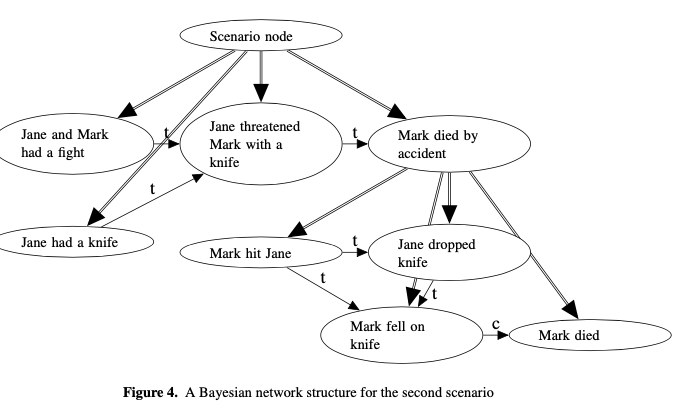
\includegraphics[width=\linewidth]{images/vlek2015.png}
\caption{Vlek BN.}
\label{vlek}
\end{center}
\end{figure}

Why to choose for subscenarios when it is not required? Tomorrow I will look up why the scenario construction was used and I will see if it does something that I miss? Coherence? But that also travels up the chain? But something with d-separation probably. I'll read the Vlek 2015 again i guess.

And then I will also reflect on the evaluation section, and also show a plot of the changing prior, and maybe do the accuracy etc.



